\apendice{Documentación de usuario}

\section{Requisitos software y hardware para ejecutar el proyecto.}
\subsection{Requisitos software}
La aplicación web se ha desarrollado de forma local, utilizando localhost, por lo cual tan sólo funcionará en un dispositivo que cumpla los siguientes requisitos:
\begin{itemize}
    \item Instalación de la aplicación XAMPP: Esta aplicación permite la utilización de un servidor local para desarrollo web. 
    \begin{itemize}
        \item Durante la utilización de la aplicación web deben estar activadas las funciones de Apache y MySQL de la app XAMPP \ref{fig:xamppactivar}, con el objetivo de garantizar un correcto funcionamiento del servidor web Apache y las bases de datos MySQL utilizadas en la app web.
    \end{itemize}
    \item Alojamiento de la carpeta que contiene los archivos de código utilizados en la aplicación web en la carpeta xampp/htdocs del dispositivo: Esto permite la inserción de los archivos en el servidor web Apache, y por tanto el acceso desde cualquier navegador a los archivos mediante un link en el siguiente formato: 
    
    'http://localhost/Nombrecarpeta/archivo.extensión'
    \item Visual Studio: Entorno de desarrollo integrado que incluye un conjunto de herramientas para el desarrollo software en diversos lenguajes de programación.
    \begin{itemize}
        \item Esta aplicación debe utilizarse para ejecutar el archivo '/bluetooth/ArduinoBridge/bridge.py', que debe estar en ejecución constante al realizar actividades con el dispositivo, sirviendo como enlace entre el Arduino y el servidor web.
    \end{itemize}
    \item Node.js: Entorno de ejecución de JavaScript que permite utilizar dicho lenguaje tanto en el lado del servidor como en el lado del cliente. Se utiliza para controlar la comunicación entre la web, el dispositivo Arduino y la base de datos.
    \begin{itemize}
        \item Este entorno nos permite ejecutar el archivo server.js mediante el comando 'node server.js', que puede ejecutarse en la terminal integrada de Visual Studio.
    \end{itemize}
    \item Arduino IDE: Aplicación necesaria para cargar los scripts Arduino en el hardware. Este proceso será explicado en detalle en el apartado 'Instalación/puesta en marcha'
\end{itemize}
\begin{figure}
    \centering
    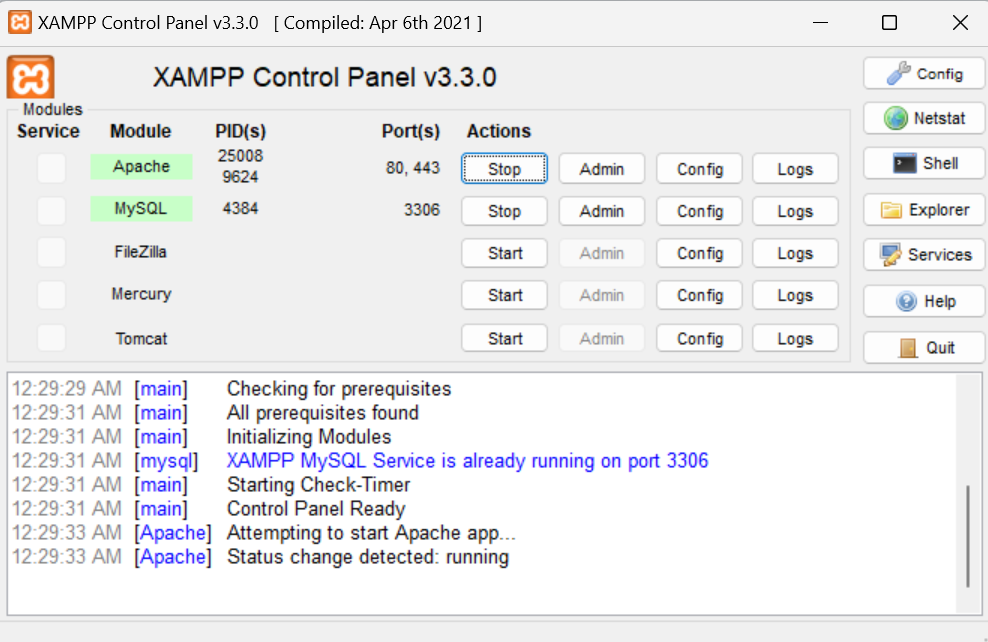
\includegraphics[width=1\textwidth]{img/xamppactivar.png}
    \caption{Pantalla de inicio de XAMPP con las funciones de Apache y MySQL activadas. Fuente propia.}
    \label{fig:xamppactivar}
\end{figure}[h]
Con el objetivo de ilustrar los requisitos funcionales con los que debe cumplir la aplicacion web para su correcto funcionamiento, se presentan una serie de tablas. Los requisitos funcionales descritos en las tablas \ref{RF-01} hasta la \ref{RF-07} han sido obtenidos del TFG \cite{Martos2024}, ya que se mantienen en la versión de la app propuesta en este proyecto. Por otro lado, los requisitos funcionales descritos en las tablas \ref{RF-08} hasta la \ref{RF-11} reflejan los requisitos funcionales nuevos.
\begin{table}[p]
    \centering
    \begin{tabularx}{\linewidth}{ p{0.21\columnwidth} p{0.71\columnwidth} }
        \toprule
        \textbf{RF-01}    & \textbf{Iniciar sesión}\\
        \toprule
        \textbf{Descripción}              & Todos los usuarios deben introducir de forma obligatoria su correo electrónico, tipo de usuario y contraseña para poder acceder a la página web.   \\
        \textbf{Importancia}                & Baja \\
        \bottomrule
    \end{tabularx}
    \caption{RF-01 Iniciar Sesión \cite{Martos2024}}
    \label{RF-01}
\end{table}

\begin{table}[p]
    \centering
    \begin{tabularx}{\linewidth}{ p{0.21\columnwidth} p{0.71\columnwidth} }
        \toprule
        \textbf{RF-02}    & \textbf{Consultar pacientes y usuarios}\\
        \toprule
        \textbf{Descripción}              & Otorgar acceso a la lista completa de usuarios o pacientes, según los permisos asignados al usuario, y permitir la realización de búsquedas específicas dentro de ella.   \\
        \textbf{Importancia}                & Media \\
        \bottomrule
    \end{tabularx}
    \caption{RF-02 Consultar pacientes y usuarios \cite{Martos2024}}
    \label{RF-02}
\end{table}

\begin{table}[p]
    \centering
    \begin{tabularx}{\linewidth}{ p{0.21\columnwidth} p{0.71\columnwidth} }
        \toprule
        \textbf{RF-03}    & \textbf{Gestionar pacientes y usuarios}\\
        \toprule
        \textbf{Descripción}              & Permitir la creación y eliminación de cuentas, así como la modificación de los datos almacenados en las cuentas de pacientes y médicos. La capacidad para realizar estas acciones depende del nivel de acceso que el usuario tenga en el sistema web.   \\
        \textbf{Importancia}                & Media \\
        \bottomrule
    \end{tabularx}
    \caption{RF-03 Gestionar pacientes y usuarios \cite{Martos2024}}
    \label{RF-03}
\end{table}

\begin{table}[p]
    \centering
    \begin{tabularx}{\linewidth}{ p{0.21\columnwidth} p{0.71\columnwidth} }
        \toprule
        \textbf{RF-04}    & \textbf{Realizar actividad}\\
        \toprule
        \textbf{Descripción}              & Ofrece las opciones de iniciar y finalizar actividades, así como la opción de guardar o descartar estas mismas.   \\
        \textbf{Importancia}                & Alta \\
        \bottomrule
    \end{tabularx}
    \caption{RF-04 Realizar actividad \cite{Martos2024}}
    \label{RF-04}
\end{table}

\begin{table}[p]
    \centering
    \begin{tabularx}{\linewidth}{ p{0.21\columnwidth} p{0.71\columnwidth} }
        \toprule
        \textbf{RF-05}    & \textbf{Mostrar actividades}\\
        \toprule
        \textbf{Descripción}              & Presenta al usuario en una lista las actividades realizadas por el paciente, permitiendo diferentes visualizaciones y llevar a cabo filtrados.   \\
        \textbf{Importancia}                & Alta \\
        \bottomrule
    \end{tabularx}
    \caption{RF-05 Mostrar actividades \cite{Martos2024}}
    \label{RF-05}
\end{table}

\begin{table}[p]
    \centering
    \begin{tabularx}{\linewidth}{ p{0.21\columnwidth} p{0.71\columnwidth} }
        \toprule
        \textbf{RF-06}    & \textbf{Consultar estadísticas}\\
        \toprule
        \textbf{Descripción}              & Visualización de los datos relacionados con las actividades realizadas por el paciente, ya sea de una actividad en concreto o de todas en conjunto.   \\
        \textbf{Importancia}                & Media \\
        \bottomrule
    \end{tabularx}
    \caption{RF-06 Consultar Estadísticas \cite{Martos2024}}
    \label{RF-06}
\end{table}

\begin{table}[p]
    \centering
    \begin{tabularx}{\linewidth}{ p{0.21\columnwidth} p{0.71\columnwidth} }
        \toprule
        \textbf{RF-07}    & \textbf{Gestionar cuenta}\\
        \toprule
        \textbf{Descripción}              & Facilitar a los usuarios las tareas de cambio de contraseña y actualización del correo eléctrónico vinculado a su cuenta.  \\
        \textbf{Importancia}                & Baja \\
        \bottomrule
    \end{tabularx}
    \caption{RF-07 Gestionar cuenta \cite{Martos2024}}
    \label{RF-07}
\end{table}

\begin{table}[p]
    \centering
    \begin{tabularx}{\linewidth}{ p{0.21\columnwidth} p{0.71\columnwidth} }
        \toprule
        \textbf{RF-08}    & \textbf{Personalizar el funcionamiento del dispositivo}\\
        \toprule
        \textbf{Descripción}              & Facilitar al usuario la realización de una prueba que permita personalizar el número de segundos que el script de Arduino identifica como congelamiento de la marcha.  \\
        \textbf{Importancia}                & Media \\
        \bottomrule
    \end{tabularx}
    \caption{RF-08 Personalizar el funcionamiento del dispositivo. Fuente propia}
    \label{RF-08}
\end{table}

\begin{table}[p]
    \centering
    \begin{tabularx}{\linewidth}{ p{0.21\columnwidth} p{0.71\columnwidth} }
        \toprule
        \textbf{RF-09}    & \textbf{Almacenar datos diarios}\\
        \toprule
        \textbf{Descripción}              & Facilitar a los usuarios de tipo 'paciente' la posibilidad de rellenar 2 formularios correspondientes a un diario de tomas de medicación y un diario de fluctuaciones motoras.  \\
        \textbf{Importancia}                & Media \\
        \bottomrule
    \end{tabularx}
    \caption{RF-09 Almacenar datos diarios. Fuente propia.}
    \label{RF-09}
\end{table}

\begin{table}[p]
    \centering
    \begin{tabularx}{\linewidth}{ p{0.21\columnwidth} p{0.71\columnwidth} }
        \toprule
        \textbf{RF-10}    & \textbf{Visualización de gráficas}\\
        \toprule
        \textbf{Descripción}              & Facilitar a los usuarios el acceso a una serie de gráficas creadas a partir de los datos almacenados sobre las actividades realizadas y los datos diarios.  \\
        \textbf{Importancia}                & Media \\
        \bottomrule
    \end{tabularx}
    \caption{RF-10 Visualización de gráficas. Fuente propia.}
    \label{RF-10}
\end{table}

\begin{table}[p]
    \centering
    \begin{tabularx}{\linewidth}{ p{0.21\columnwidth} p{0.71\columnwidth} }
        \toprule
        \textbf{RF-11}    & \textbf{Descarga de informe}\\
        \toprule
        \textbf{Descripción}              & Facilitar a los usuariosde tipo 'profesional' la descarga de un informe en PDF conteniendo información relevante sobre el paciente, sus actividades realizadas y de forma opcional las gráficas.  \\
        \textbf{Importancia}                & Baja \\
        \bottomrule
    \end{tabularx}
    \caption{RF-11 Visualización de gráficas. Fuente propia.}
    \label{RF-11}
\end{table}
\subsection{Requisitos hardware}
Para asegurar el correcto funcionamiento del dispositivo es necesario que el cinturón y la tobillera contengan un circuito configurado de forma correcta, tal como se indica en el Anexo E, mediante la figura \ref{fig:esquemahardware}, y conteniendo los siguientes componentes:
\begin{itemize}
    \item Microcontrolador Arduino UNO3, conectado a un Arduino proto shield que posibilita la conexión de múltiples cables a cada pin de la placa Arduino UNO.
    \item Fuente de alimentación recargable 9V, conectada a la placa mediante un cable adaptador de bateria Arduino DC 9V.
    \item Interruptor ON/OFF.
    \item 2 pulsadores 'start' y 'stop'
    \item Módulo bluetooth HC-05, necesario para la comunicación bidireccional con el servidor web.
    \item Pantalla de display LCD 16x2 con Interfaz I2C 2x16 incorporada, la cual facilita una conexión más sencilla, utilizando tan solo 4 cables.
    \item Sensor acelerómetro y giroscopio MPU-6050.
    \item Cable multihilo, conectado a los cables provenientes de la placa mediante un conector macho-hembra.
    \item Cables de calibre 28 AWG (en total unos 3m) para la conexión de los diferentes componentes a la placa Arduino.
\end{itemize}
\section{Instalación / Puesta en marcha}
\subsection{Puesta en marcha del dispositivo Arduino}
\begin{enumerate}
    \item Calibración del dispositivo: El primer paso para asegurar un correcto funcionamiento del dispositivo es calibrar el sensor MPU-6050 mediante el script de calibración 'calibracionDMP.ino'. Para ello se conectará por cable la placa Arduino UNO del dispositivo con el ordenador en que tengamos este script. Utilizando la aplicación Arduino IDE cargamos el script en la placa, tal como muestra la figura \ref{fig:cargascript}.
    \begin{figure}[h]
        \centering
        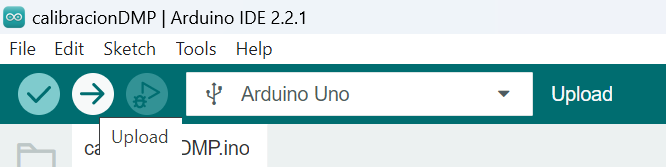
\includegraphics[width=1\textwidth]{img/cargascript.png}
        \caption{Carga del script 'calibracionDMP.ino' utilizando Arduinio IDE. Fuente propia.}
        \label{fig:cargascript}
    \end{figure}
    Tras la carga del script, manteniendo la conexión por cable con la placa, es necesario abrir la función 'Serial Monitor' de Arduino IDE, en la cual observaremos la comunicación serial con el dispositivo Arduino. Será necesario enviar un carácter cualquiera para iniciar el proceso de calibración, y al finalizar el proceso obtendremos unos resultados \ref{fig:calibracion}.
    \begin{figure}[h]
        \centering
        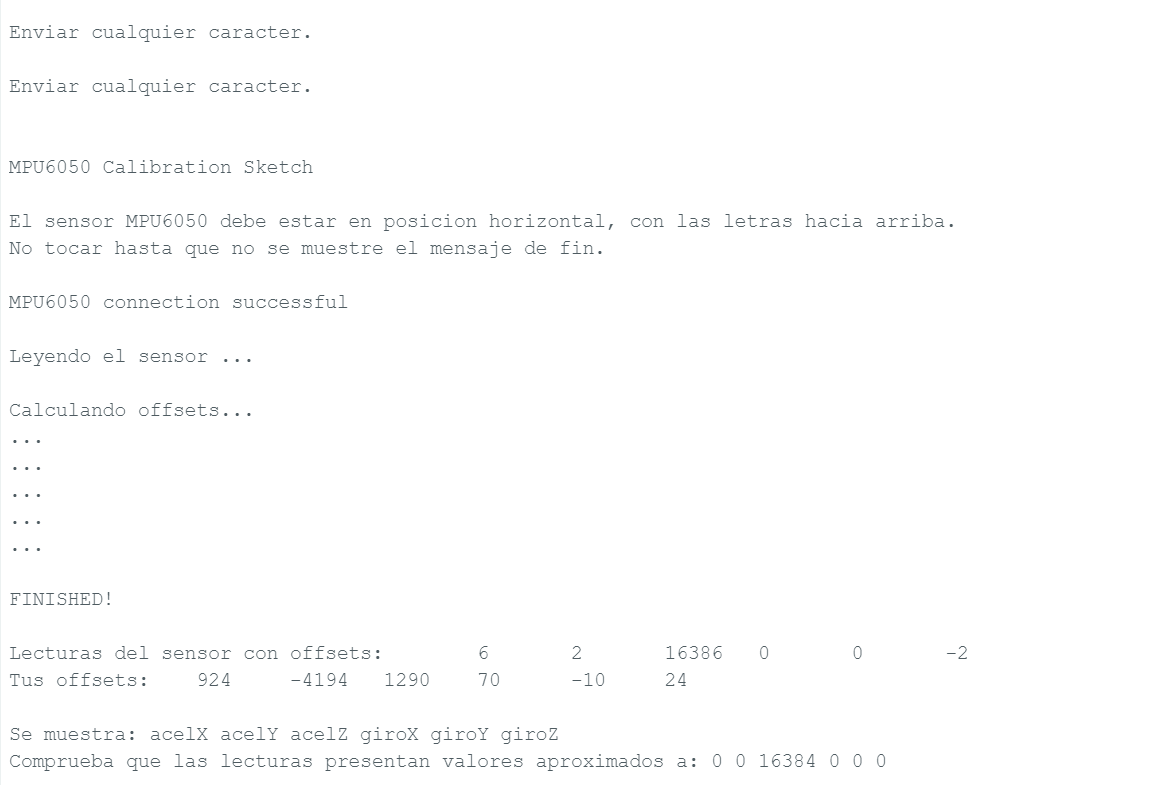
\includegraphics[width=1\textwidth]{img/calibracion.png}
        \caption{Monitor serial de Arduino IDE durante una calibración exitosa. Fuente propia.}
        \label{fig:calibracion}
    \end{figure}
    \item Carga del script: Tras haber calibrado exitosamente el sensor MPU-6050, se debe sustituir el script de calibración por el script general (en este caso la versión 5 que tiene como título laser), que contiene el programa para el funcionamiento del dispositivo. Teniendo la placa conectada por cable cargaremos el script y posteriormente podremos desconectar el cable. El dispositivo está listo para funcionar.
\end{enumerate}
\subsection{Instalación y puesta en marcha de la aplicación web}
\begin{enumerate}
    \item Tras asegurarnos de que en el ordenador a utilizar se cumplen los requisitos software previamente mencionados (instalación de la apicación XAMPP y de Visual Studio Code, alojamiento de la carpeta con archivos de código en xampp/htdocs, instalación de Node.js y ejecución de las funciones Apache y MySQL de XAMPP) deberíamos ser capaces de acceder a la app insertando el link en cualquier navegador del dispositivo:
    
    \url{http://localhost/Web_VisualStudio/common/login.html} 
    \item Para utilizar las funciones de la app que implican conexión en tiempo real con el dispositivo (realización de actividades y prueba de personalización), debemos seguir unos pasos adicionales:
    \begin{itemize}
        \item Conectar el dispositivo, con nombre 'TFG1', al ordenador (para cambiar la configuración del módulo bluetooth y mostrarse con otro nombre u contraseña se puede conectar el pin enable, que normalmente queda libre, al pin 5V de la placa Arduino y utilizar un script de Arduino para ello)
        \item Abrir la carpeta de archivos de código en Visual Studio Code y ejecutar el comando 'node server.js' en la terminal integrada de la carpeta ArduinoServer. De esta forma pondremos en marcha el servidor. En la figura \ref{fig:servidor} observamos una activación exitosa del servidor.
            \begin{figure}[h]
                \centering
                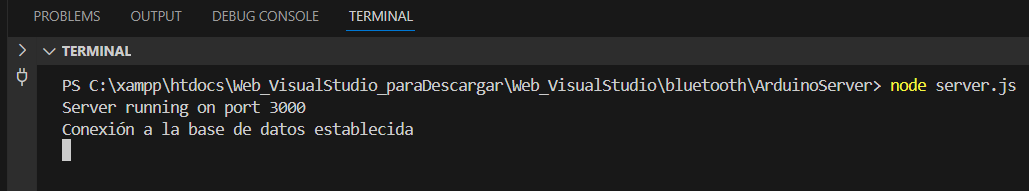
\includegraphics[width=1\textwidth]{img/servidor.png}
                \caption{Activación del servidor exitosa. Fuente propia.}
                \label{fig:servidor}
            \end{figure}
        \item Ejecutar el archivo 'bridge.py', ajustando el puerto serial según el puerto al que esté conectado el dispositivo bluetooth \ref{fig:bridgepy}. Usualmente este puerto es 'COM3' o 'COM4', pero podemos cocnsultar qué puerto se está utilizando en el administrador de dispositivos \ref{fig:admintareas}, pulsando en los puertos bluetooth y consultando en el apartado 'eventos' la conexión de dispositivos a los mismos. Tras ajustar el puerto, al ejecutar el archivo deberíamos recibir en la terminal algo similar a lo mostrado en la figura \ref{fig:bridgeejecutando} de forma continuada. En caso de observar algo distinto, es indicación de que el servidor no funciona correctamente (habría que repetir el paso anterior) o de que el puerto especificado no es el correcto.
            \begin{figure}[h]
                \centering
                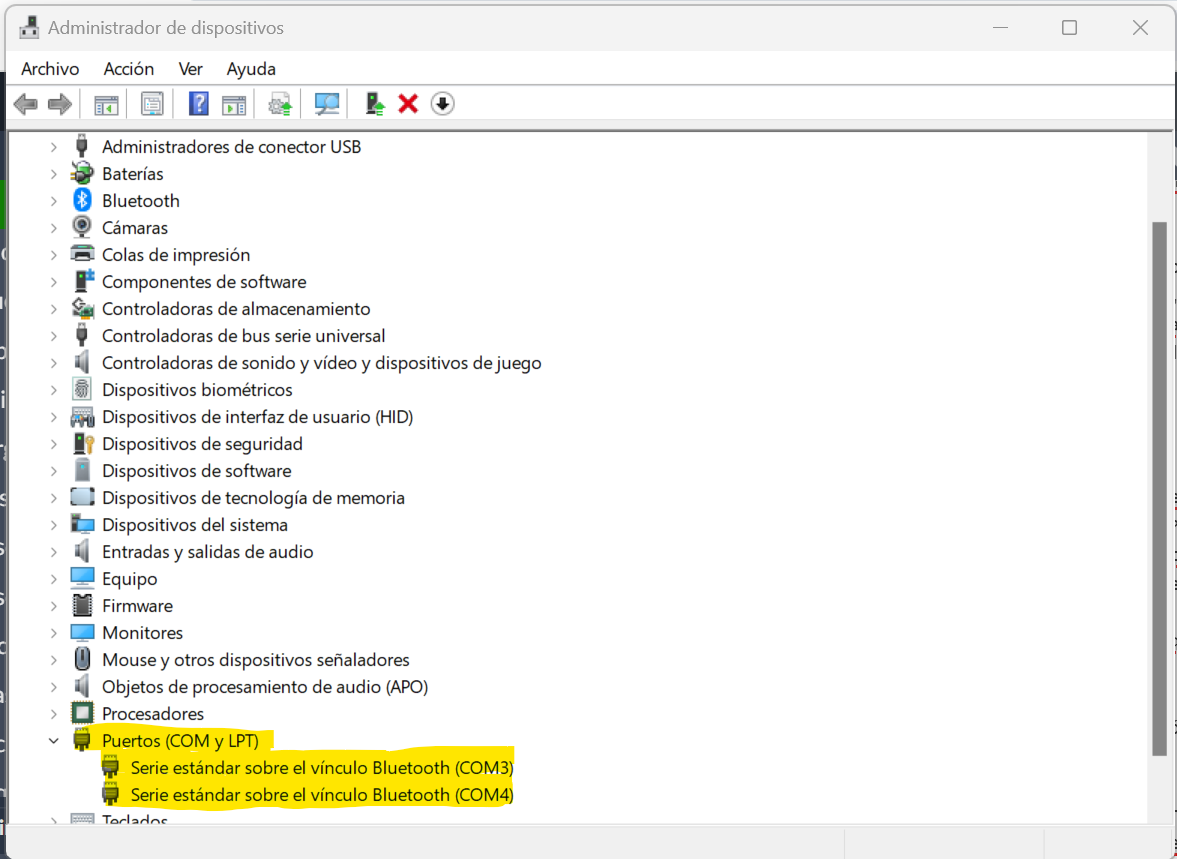
\includegraphics[width=1\textwidth]{img/admindispositivos.png}
                \caption{Consulta en el administrador de dispositivos. Fuente propia.}
                \label{fig:admintareas}
            \end{figure}
            \begin{figure}[h]
                \centering
                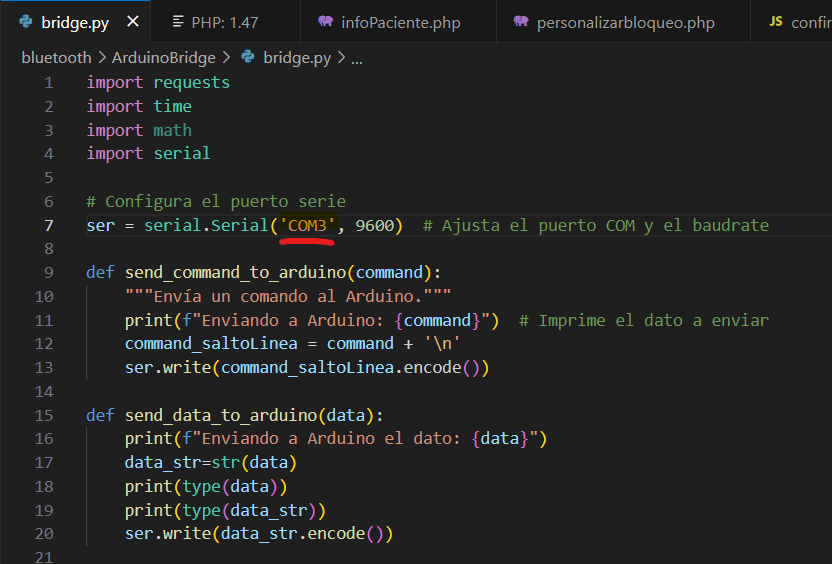
\includegraphics[width=1\textwidth]{img/bridgepy.png}
                \caption{Archivo bridge.py en que se especifica el puerto serial al que está conectado el dispositivo. Fuente propia.}
                \label{fig:bridgepy}
            \end{figure}
            \begin{figure}[h]
                \centering
                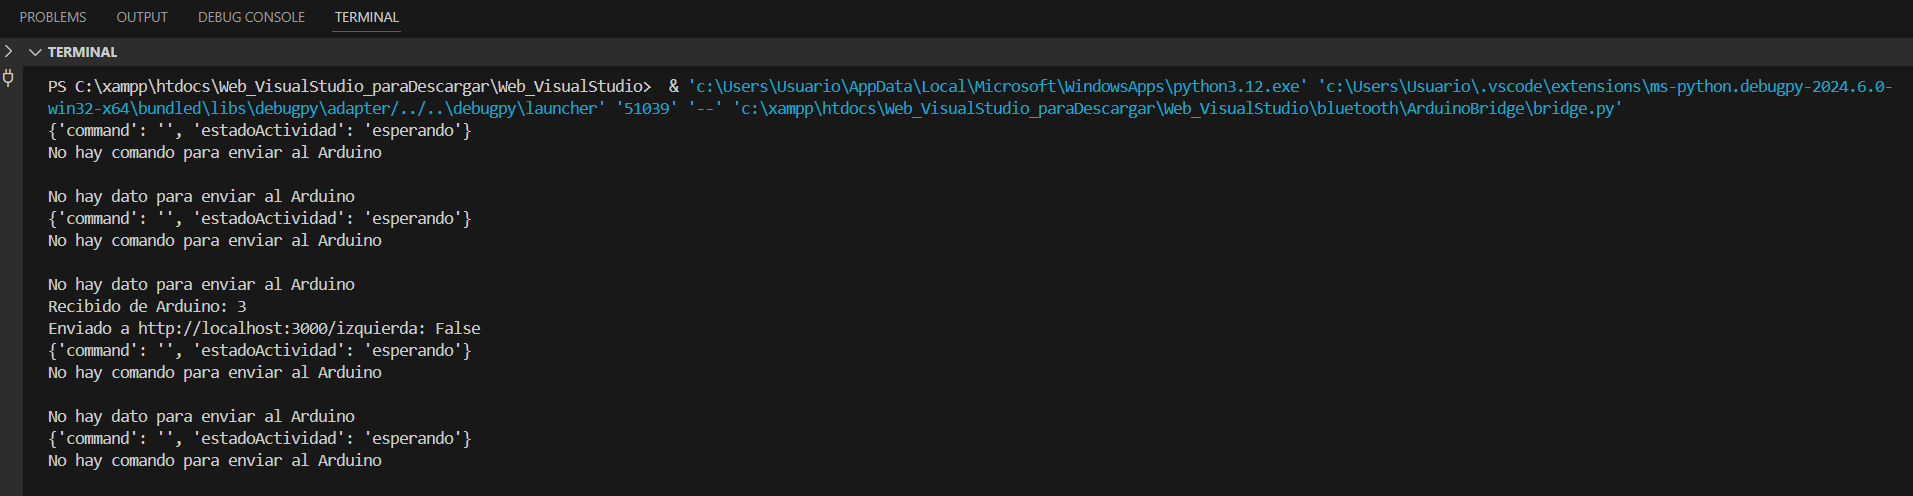
\includegraphics[width=1\textwidth]{img/bridgeejecutando.png}
                \caption{Teminal durante la ejecución exitosa del archivo bridge.py . Fuente propia.}
                \label{fig:bridgeejecutando}
            \end{figure}
    \end{itemize}
\end{enumerate}
\section{Manuales y/o Demostraciones prácticas}
Con el objetivo de clarificar el modo de uso y funcionamiento de las nuevas funciones implementadas en la aplicación web se muestran a continuación unas instrucciones para el uso de la aplicación por parte de los diferentes usuarios, así como unas indicaciones para el acceso a videos de demostración del funcionamiento de estas funciones.
\subsection{Instrucciones para el uso de las nuevas funciones en la aplicación web}
La pantalla de acceso a la aplicación web, en la que observamos un formulario de log-in se muestra en la figura \ref{fig:inicio}. Rellenando el formulario con unas credenciales válidas de un usuario con cuenta registrada en la aplicación obtendremos el acceso a la app con las funciones correspondientes a cada tipo de usuario.
\begin{figure}[h]
    \centering
    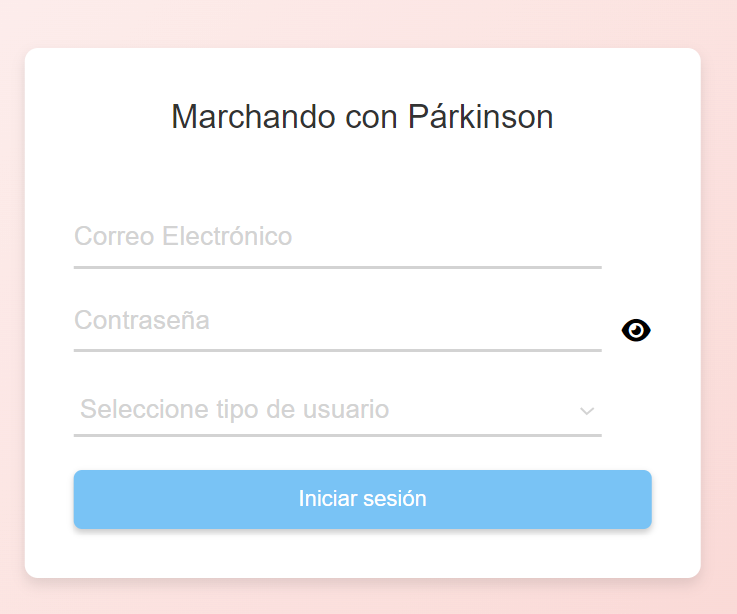
\includegraphics[width=1\textwidth]{img/inicio.png}
    \caption{Inicio de sesión en la aplicación web. Fuente propia.}
    \label{fig:inicio}
\end{figure}
Al iniciar sesión con una cuenta de tipo 'profesional', accederemos a la pantalla de inicio mostrada en la figura \ref{fig:inicioprof}, desde donde tendremos acceso al menú de navegación del profesional, y a la lista de pacientes asignados. 
\begin{figure}[h]
    \centering
    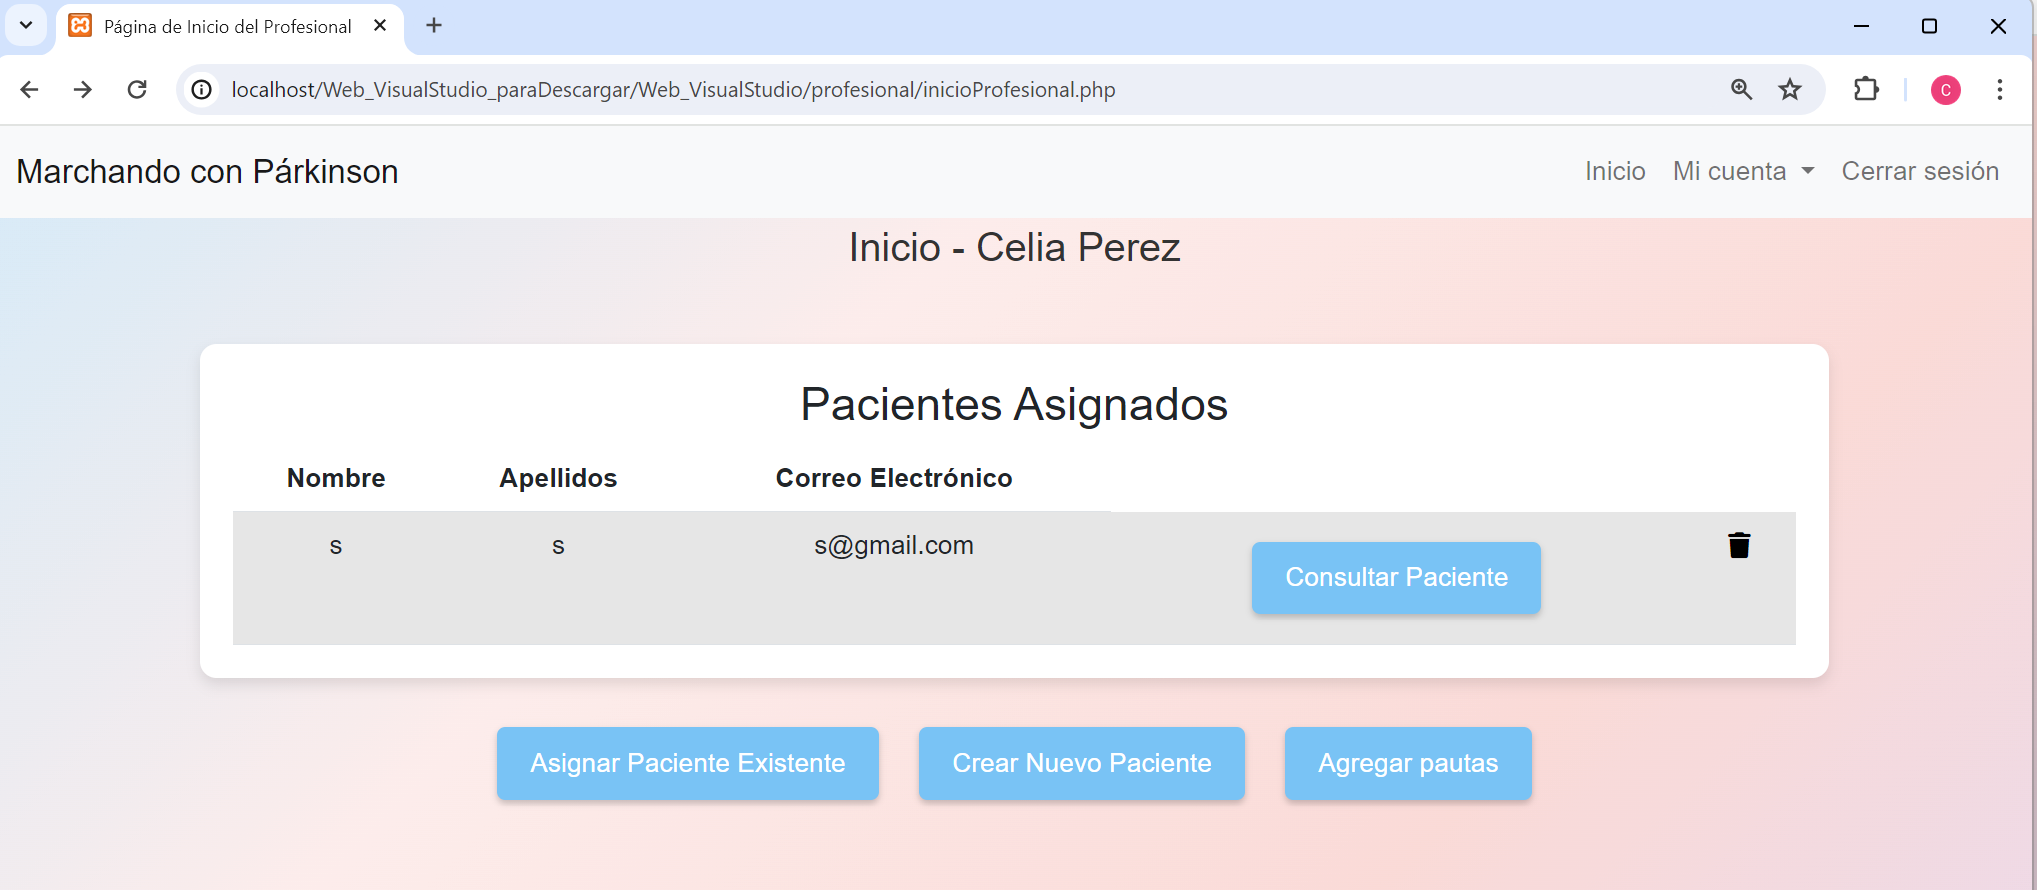
\includegraphics[width=1\textwidth]{img/inicioprof.png}
    \caption{Pantalla de inicio del usuario de tipo 'profesional'. Fuente propia.}
    \label{fig:inicioprof}
\end{figure}

Pulsando en el botón 'Agregar pautas' visualizamos el formulario para agregar una pauta a un paciente \ref{fig:pautasprof}. Para ello debemo seleccionar el ID del paciente a guardar, el número de medicaciones diferentes relacionadas con los síntomas motores del párkinson que el paciente toma cada día y rellenar los datos correspondientes a cada una de esas medicaciones (número de tomas y nombre). Estos datos aparecerán de forma predeterminada como respuestas en el diario de tomas de medicaciones del paciente.

\begin{figure}[h]
    \centering
    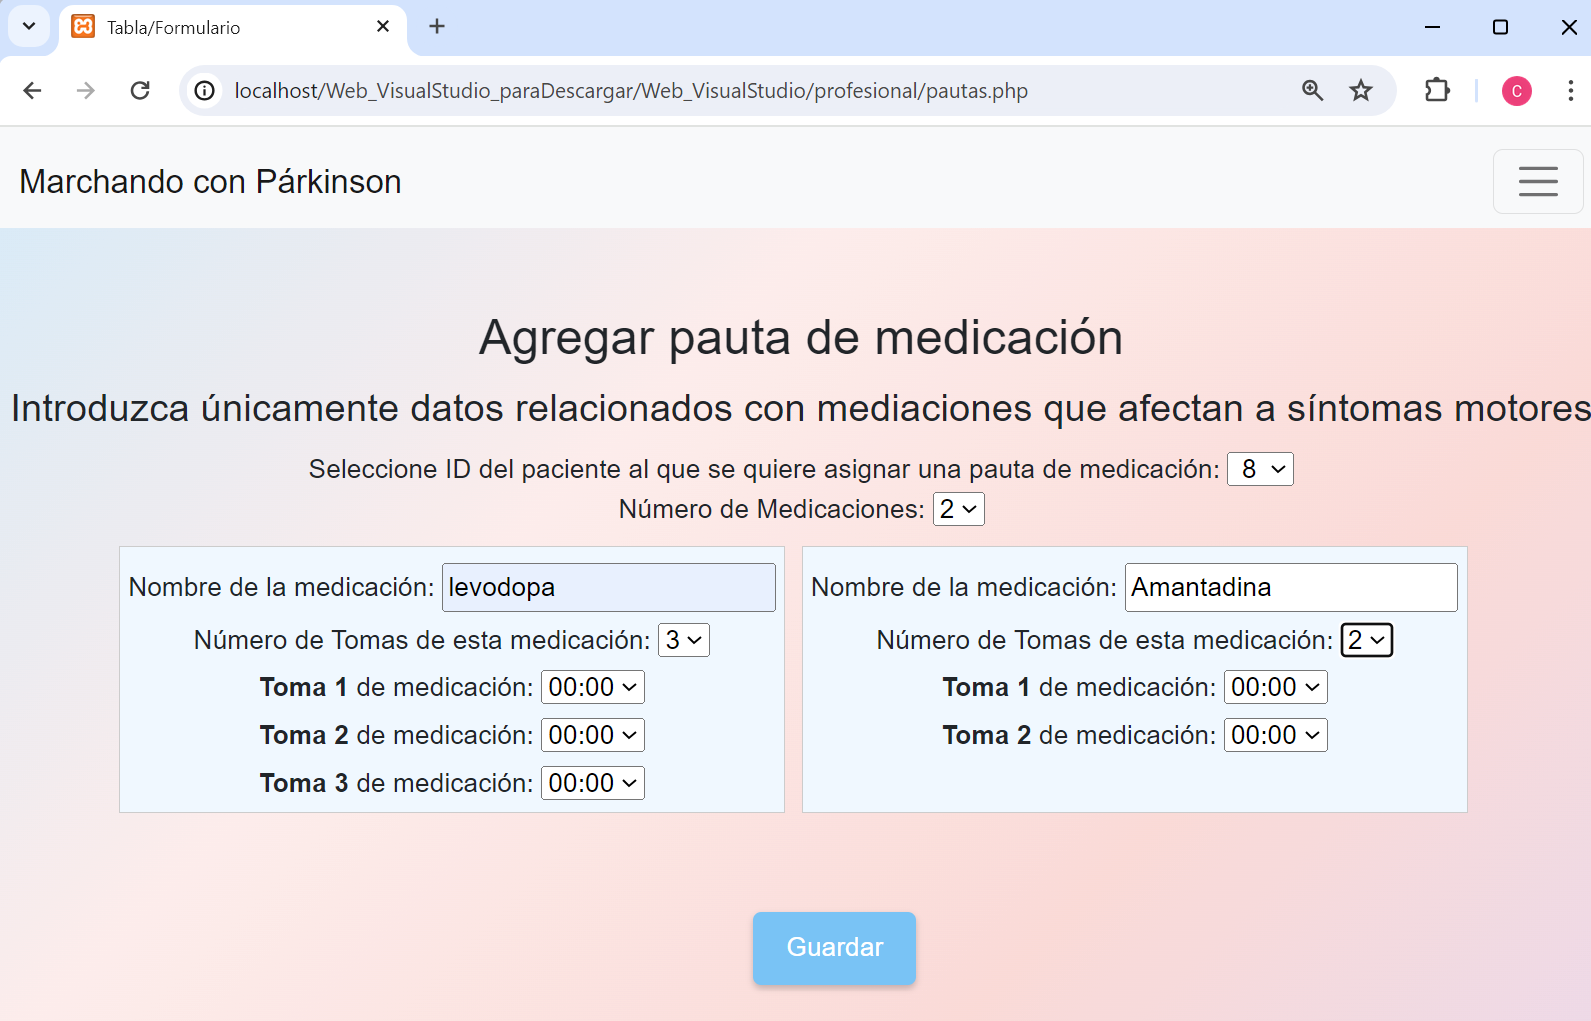
\includegraphics[width=1\textwidth]{img/pautasprof.png}
    \caption{Formulario de asignación de una pauta de medicación a un paciente por parte del profesional. Fuente propia.}
    \label{fig:pautasprof}
\end{figure}
Desde la pantalla de inicio de tipo 'profesional' también podemos consultar los datos almacenados para los pacientes asignados al usuario, desde la pantalla \ref{fig:profverpaciente}. Desde aquí podemos acceder a la prueba de personalización, cuyo funcionamiento se detalla en los videos de demostración y a las actividades y estadísticas del paciente. 

\begin{figure}[h]
    \centering
    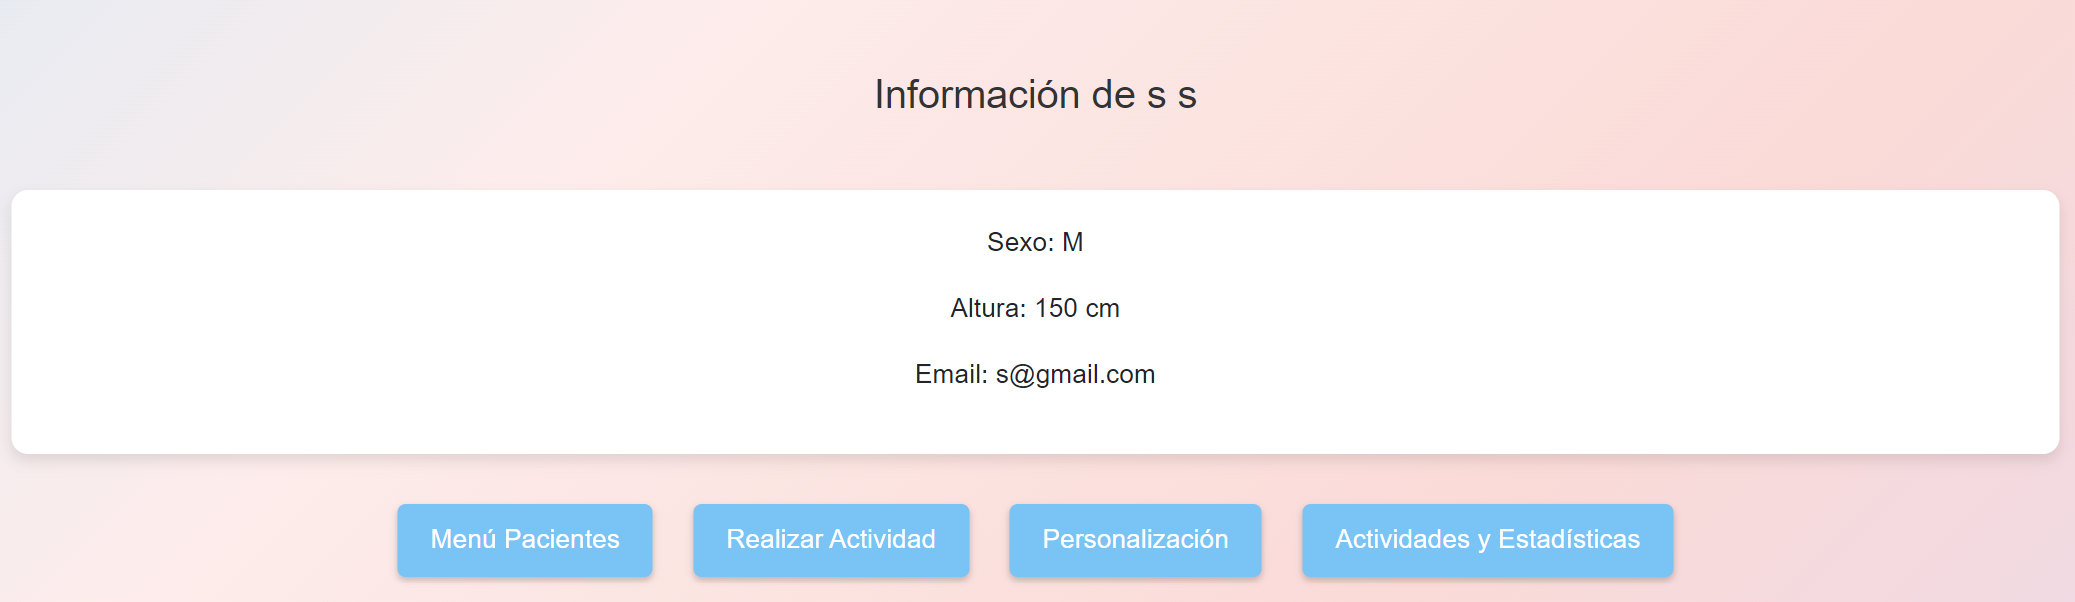
\includegraphics[width=1\textwidth]{img/profverpaciente.png}
    \caption{Consulta de un paciente asignado por parte del profesional. Fuente propia.}
    \label{fig:profverpaciente}
\end{figure}

La prueba de personalización tiene como objetivo guardar durante el comienzo del uso del dispositivo por parte del paciente un número de segundos personalizado a partir de los cuales se detectará un congelamiento de la marcha. Esto se realizará a partir de los segundos que tarde el usuario en dar 1 paso. La prueba se realizará con ayuda del profesional para asegurar su validez, por lo que se encuentra dentro de las funciones del usuario 'profesional'.

Desde el apartado de 'Actividades y Estadísticas' \ref{fig:profestadisticas}, el profesional puede descargar un informe en pdf sobre los datos de las actividades y de forma opcional las gráficas \ref{fig:pdf} o consultar de forma directa las gráficas \ref{fig:graficas}. Para observar los diferentes tipos de gráficas que pueden observarse en este apartado consultar los vídeos de demostraciones.

\begin{figure}[h]
    \centering
    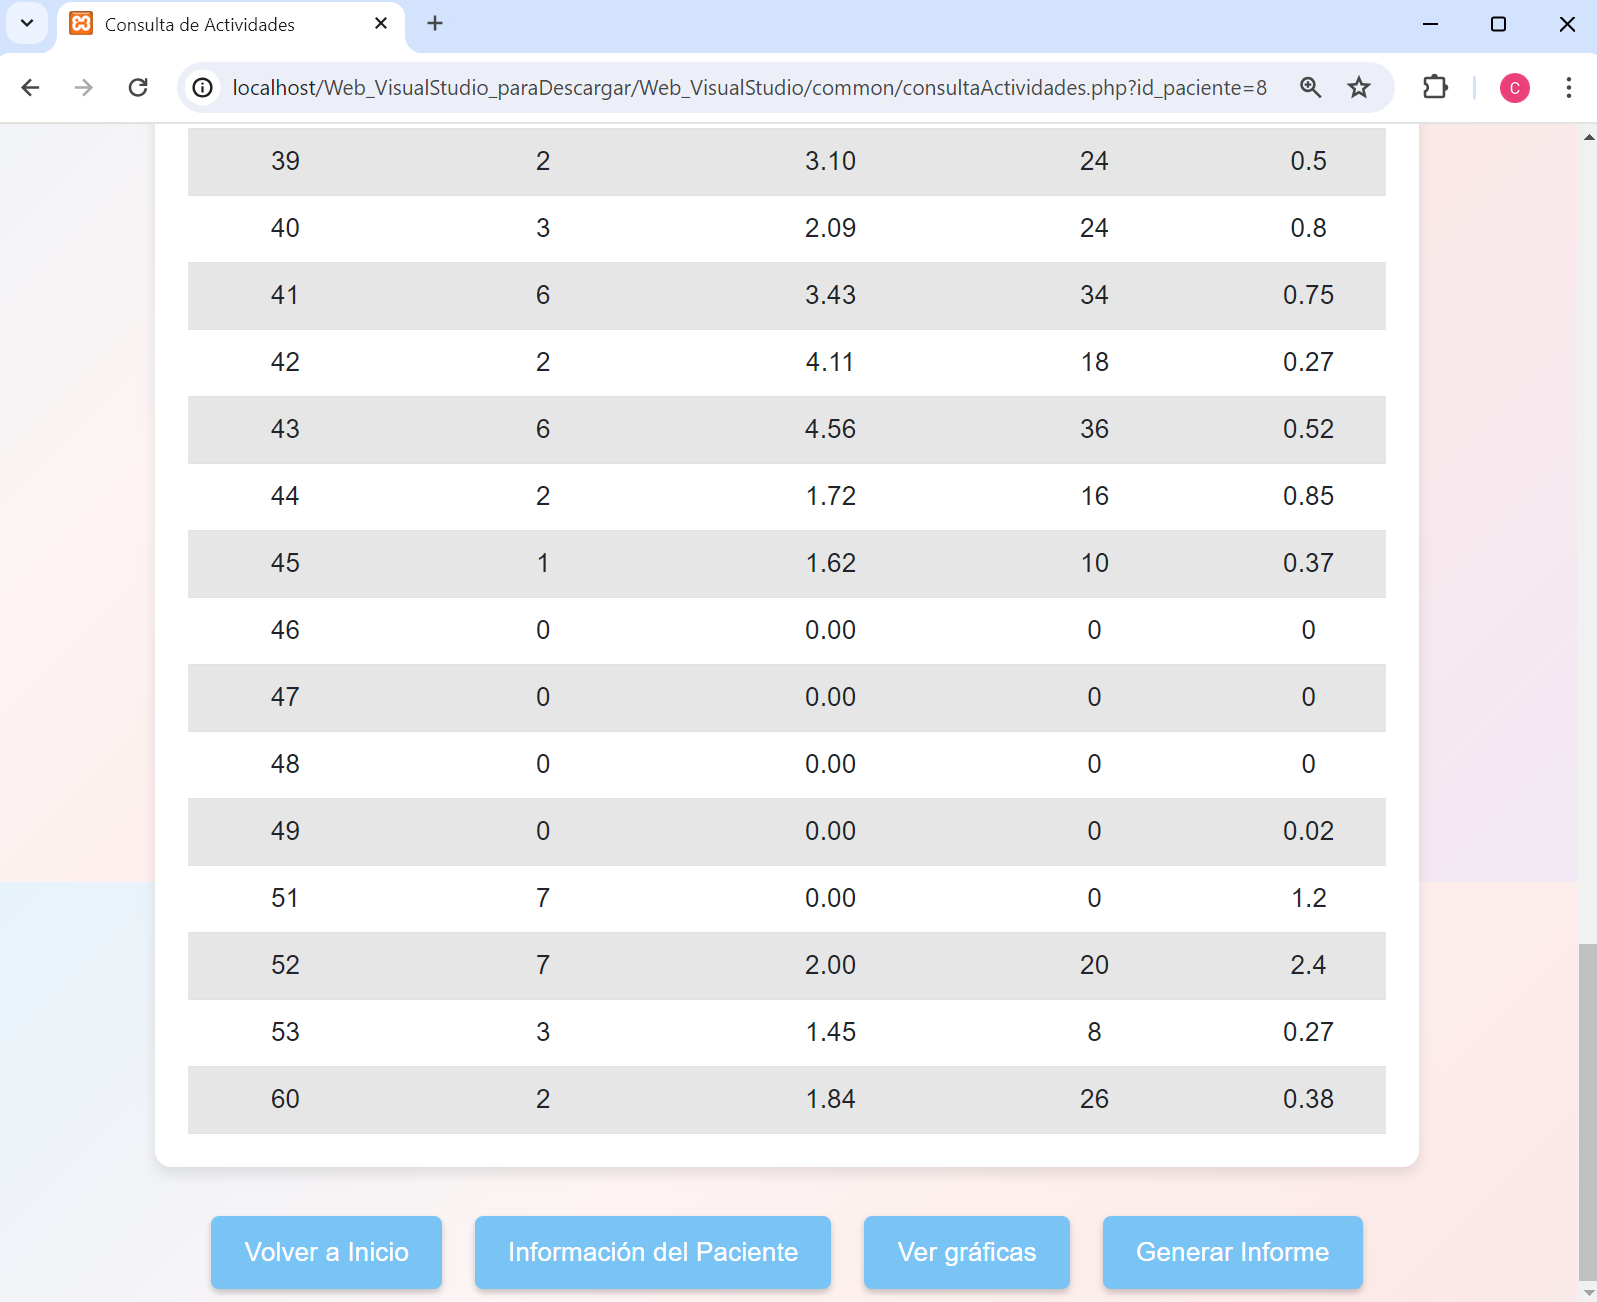
\includegraphics[width=1\textwidth]{img/profestadisticas.png}
    \caption{Vista desde el usuario 'profesional' al apartado de actividades y estadísticas de un paciente asignado. Fuente propia.}
    \label{fig:profestadisticas}
\end{figure}


\begin{figure}[h]
    \centering
    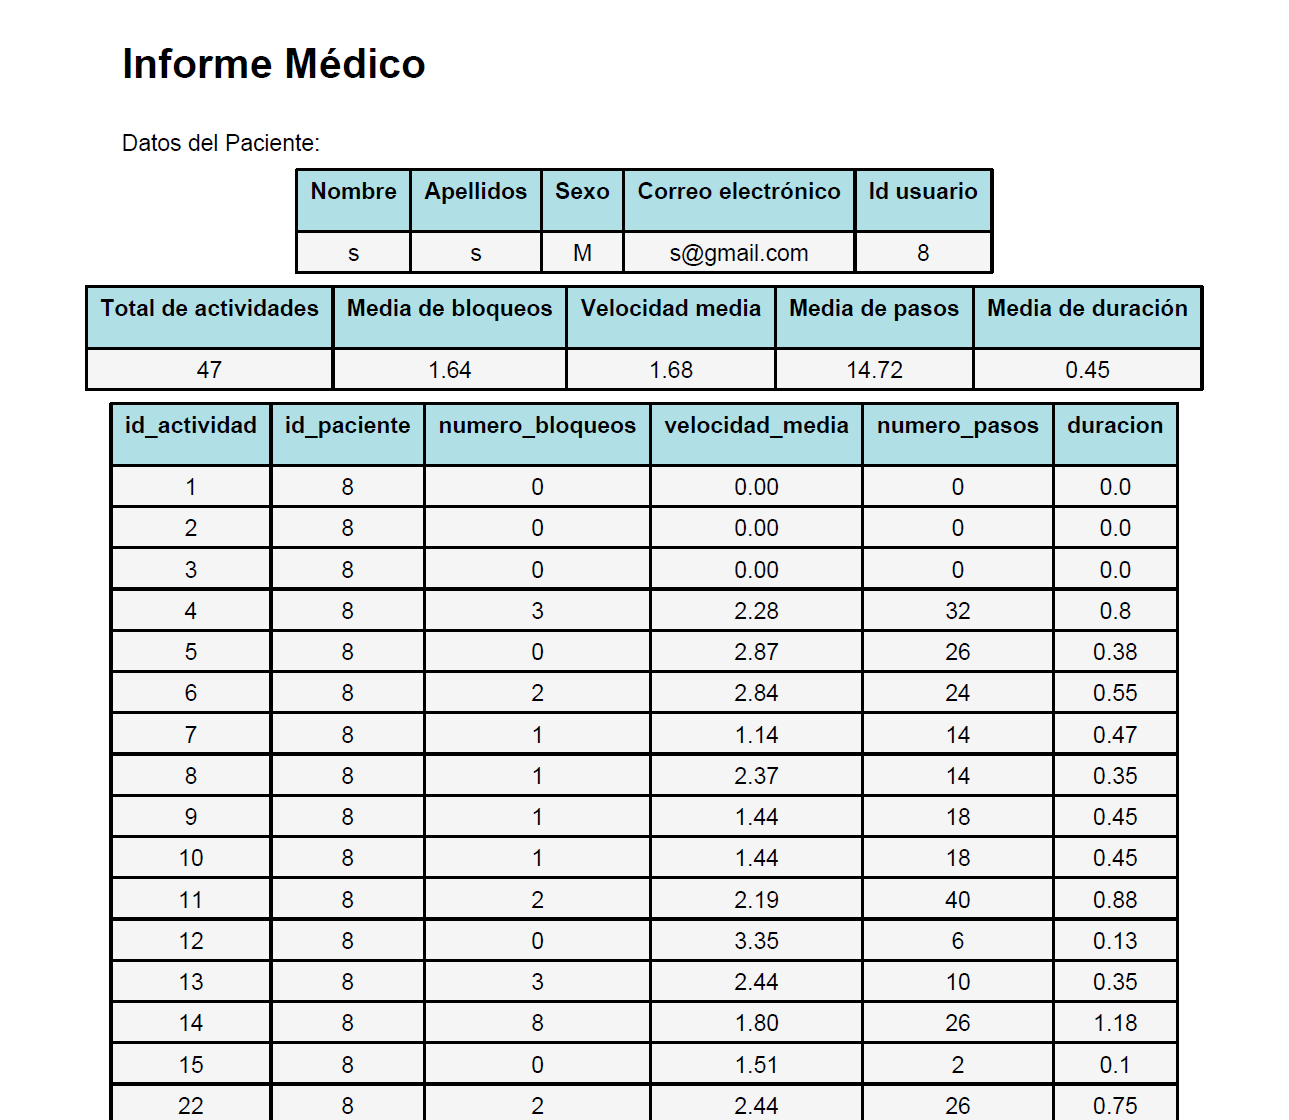
\includegraphics[width=1\textwidth]{img/pdf.png}
    \caption{Pdf generado automáticamente con los datos del paciente. Fuente propia.}
    \label{fig:pdf}
\end{figure}

\begin{figure}[h]
    \centering
    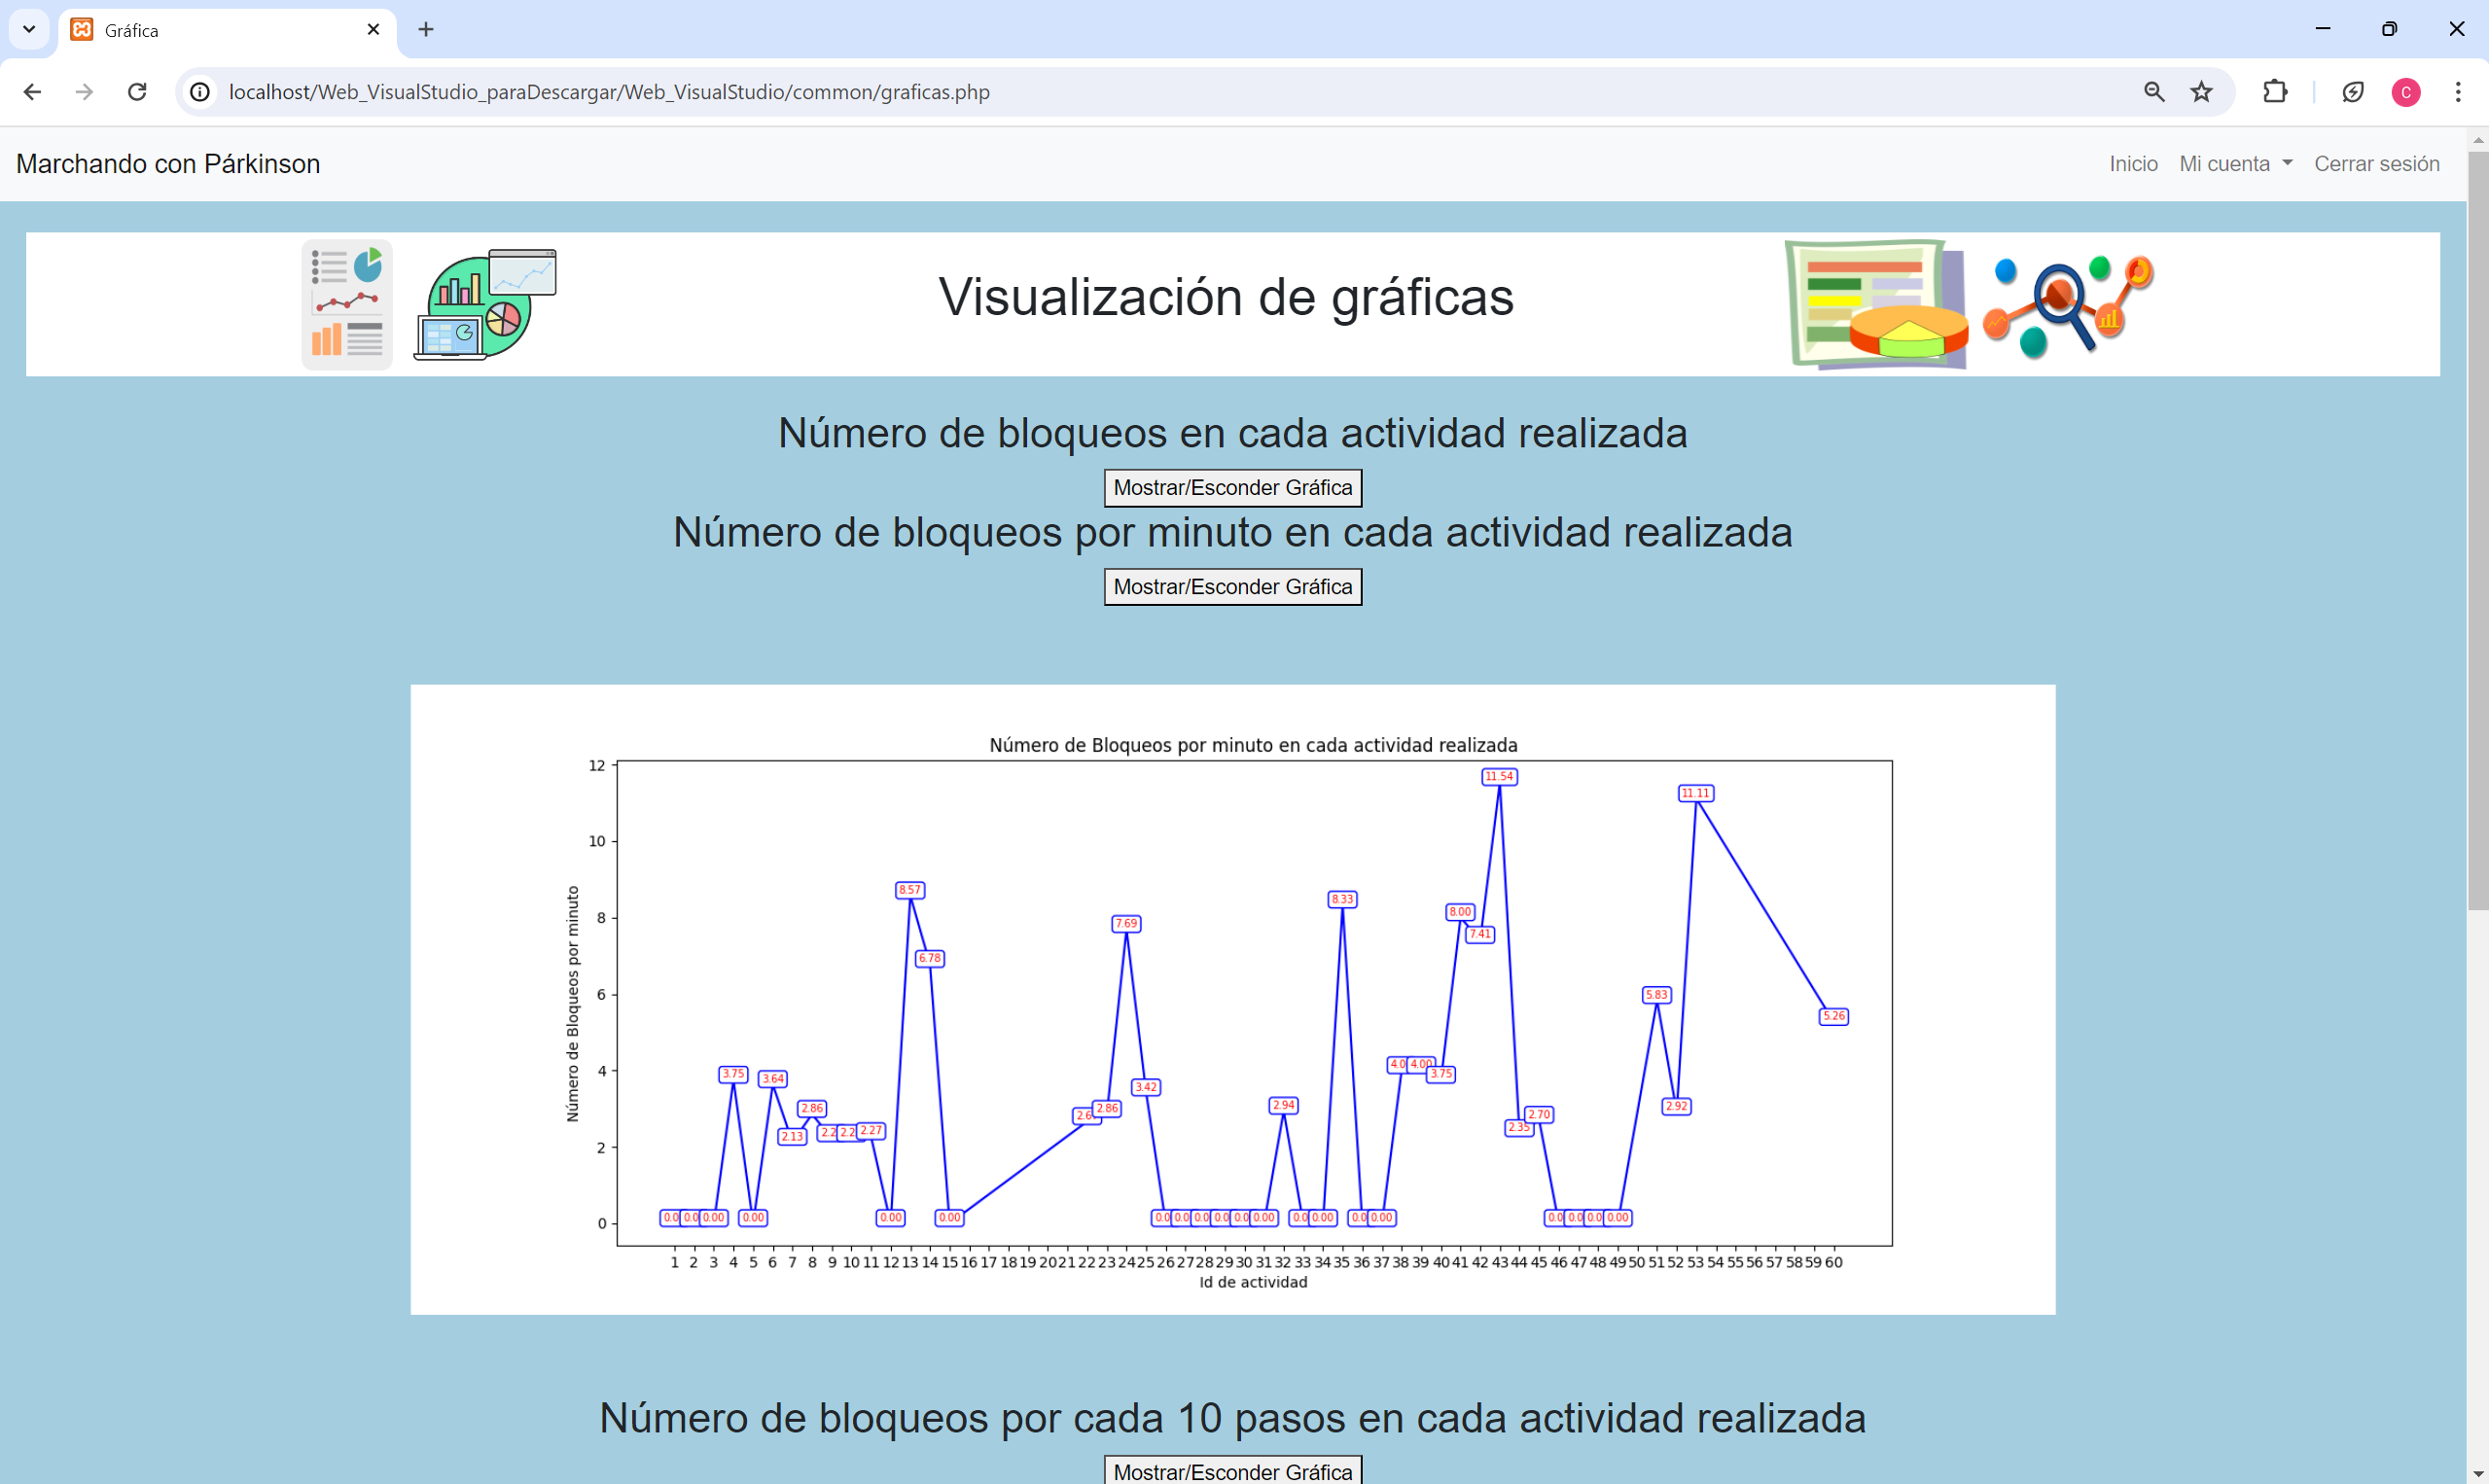
\includegraphics[width=1\textwidth]{img/graficas.png}
    \caption{Vista de las gráficas. Fuente propia.}
    \label{fig:graficas}
\end{figure}

Al acceder a la aplicación con una cuenta de tipo 'paciente', observamos la pantalla mostrada en la figura \ref{fig:iniciopaciente}. En la barra de navegación, observamos un botón 'Acceder al diario', que nos lleva a la pantalla mostrada en la figura \ref{fig:diarios}, a partir de la cual se puede acceder al diario de fluctuaciones (un diario de Hauser, tal como se describe en la memoria de este proyecto) \ref{fig:diariofluc} y al diario de tomas de medicaciones \ref{fig:diariotomas}. En este último diario observaremos como respuestas predeterminadas las correspondientes a la pauta de medicación asignada, en caso de que el profesional encargado la haya insertado como se indicó anteriormente.

\begin{figure}[h]
    \centering
    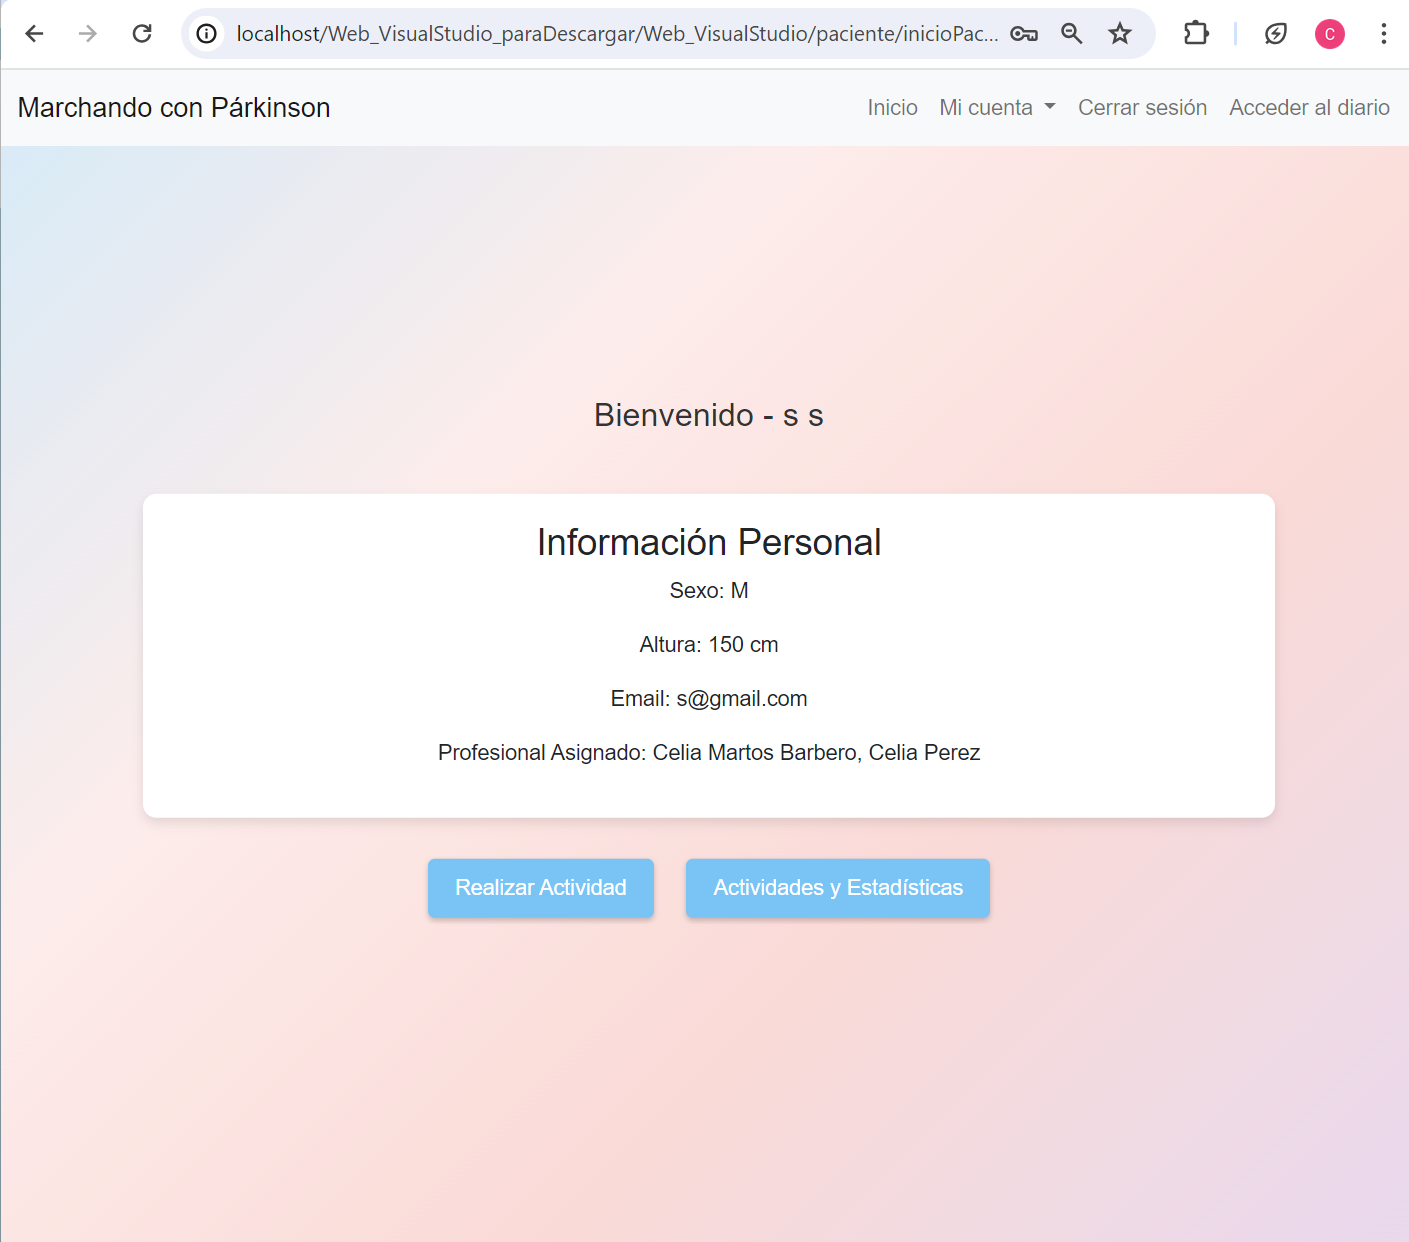
\includegraphics[width=1\textwidth]{img/iniciopaciente.png}
    \caption{Pantalla de inicio del usuario de tipo 'paciente'. Fuente propia.}
    \label{fig:iniciopaciente}
\end{figure}

\begin{figure}[h]
    \centering
    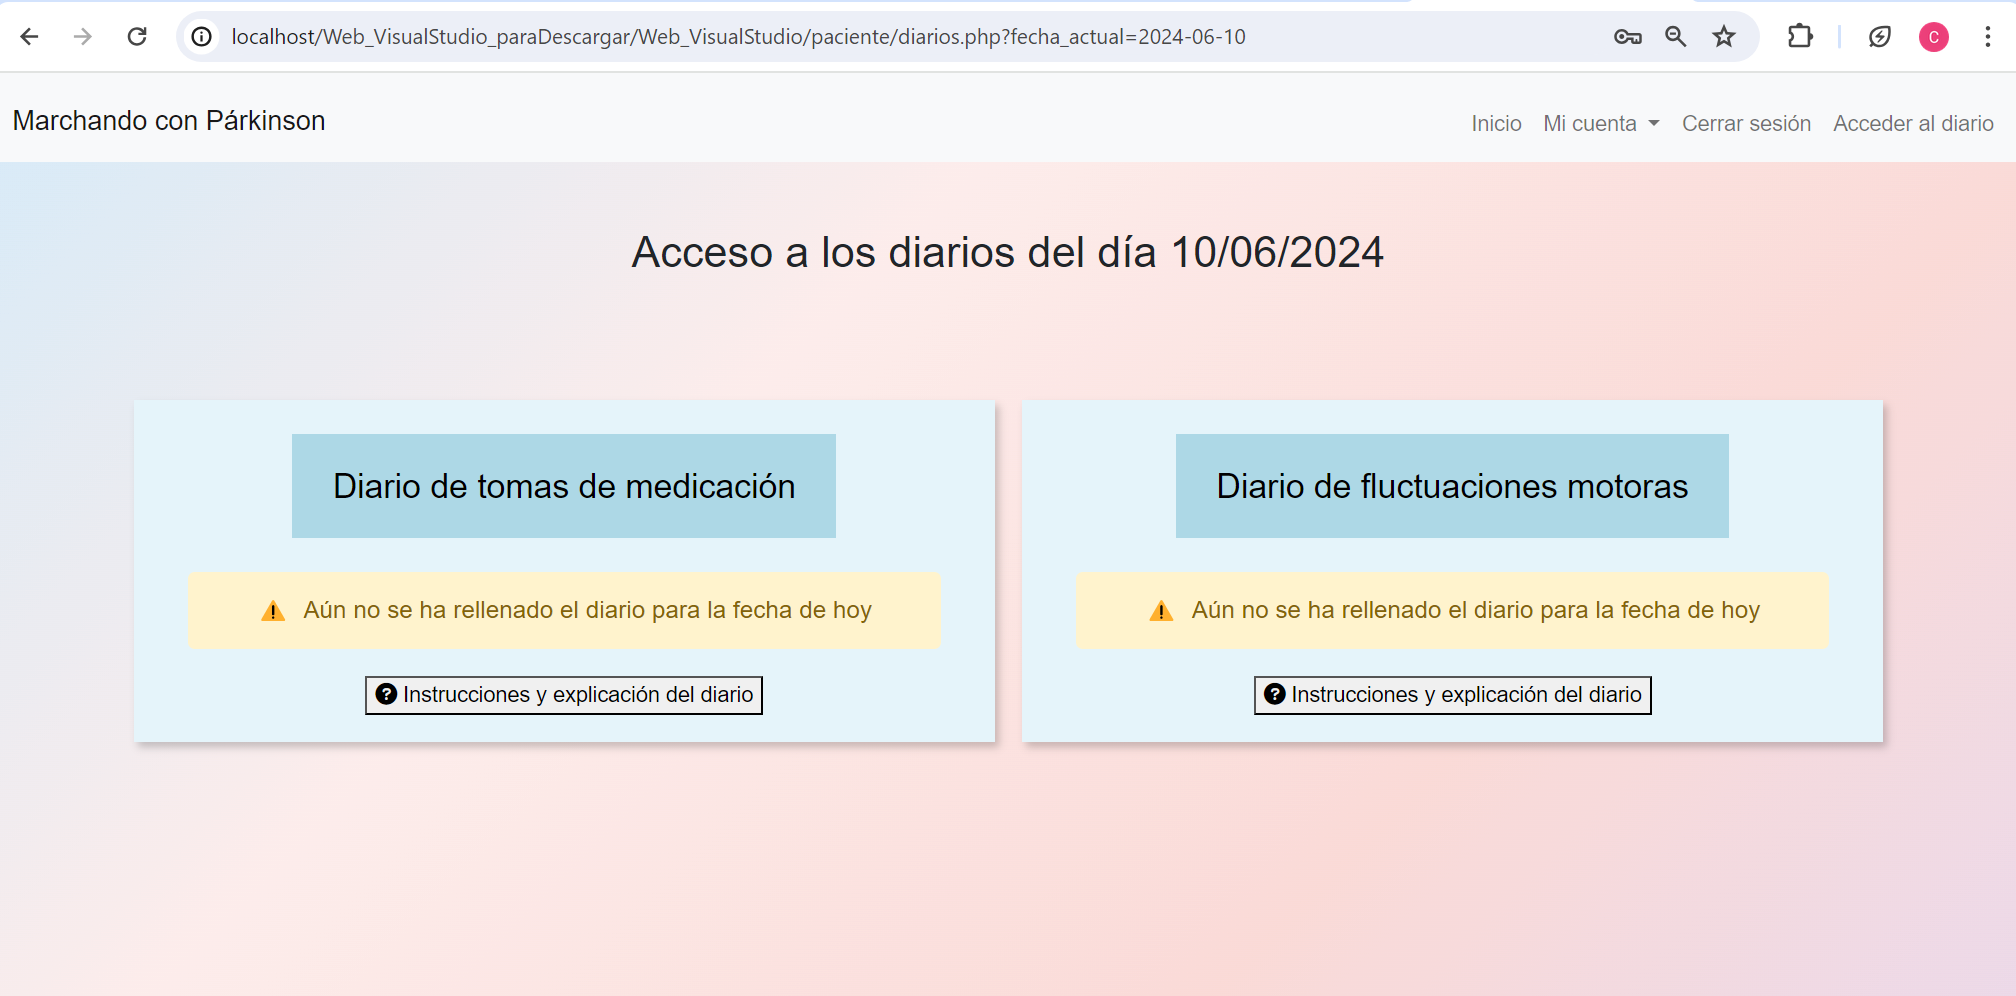
\includegraphics[width=1\textwidth]{img/diarios.png}
    \caption{Pantalla de acceso a los diarios del paciente. Fuente propia.}
    \label{fig:diarios}
\end{figure}

\begin{figure}[h]
    \centering
    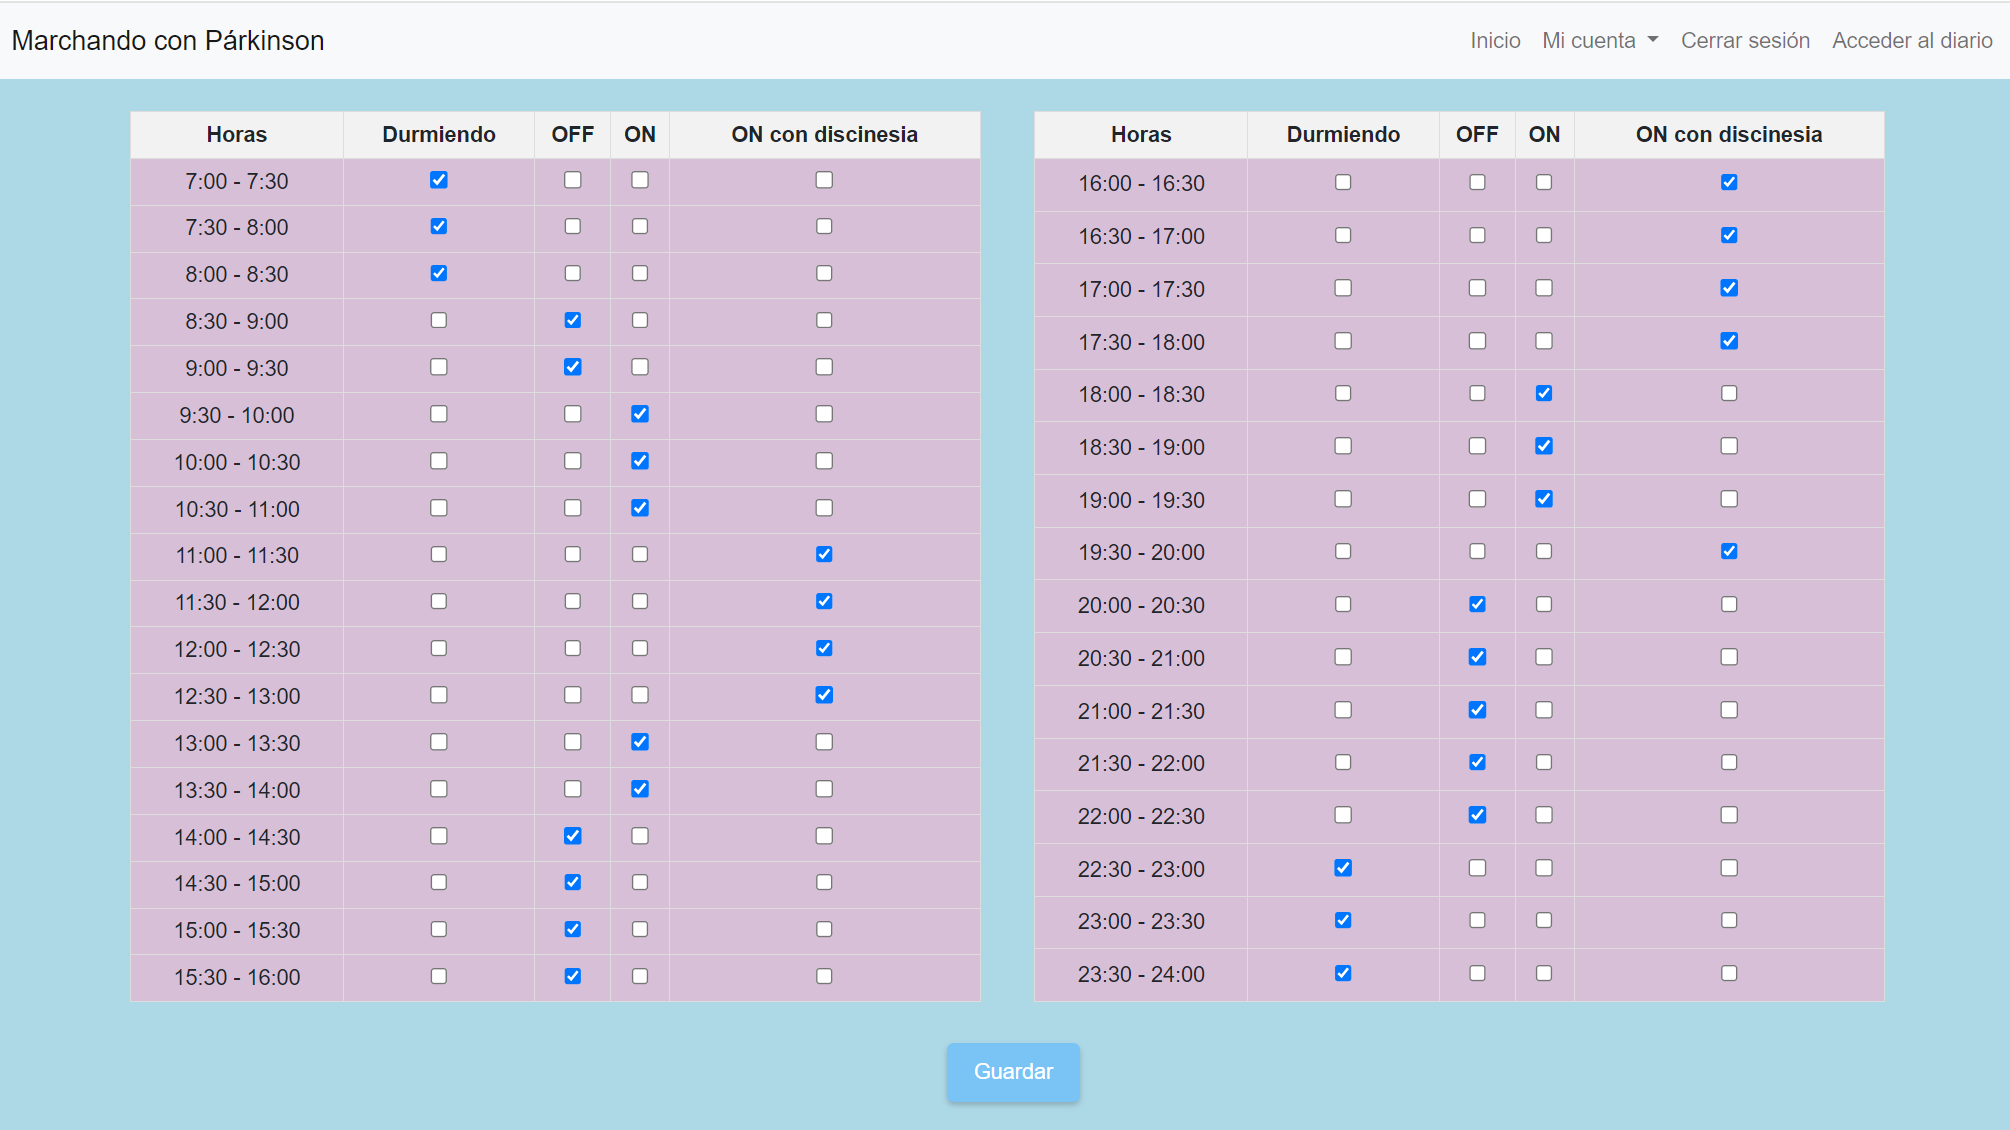
\includegraphics[width=1\textwidth]{img/diariofluc.png}
    \caption{Formulario para rellenar el diario de fluctuaciones (diario de Hauser). Fuente propia.}
    \label{fig:diariofluc}
\end{figure}

\begin{figure}[h]
    \centering
    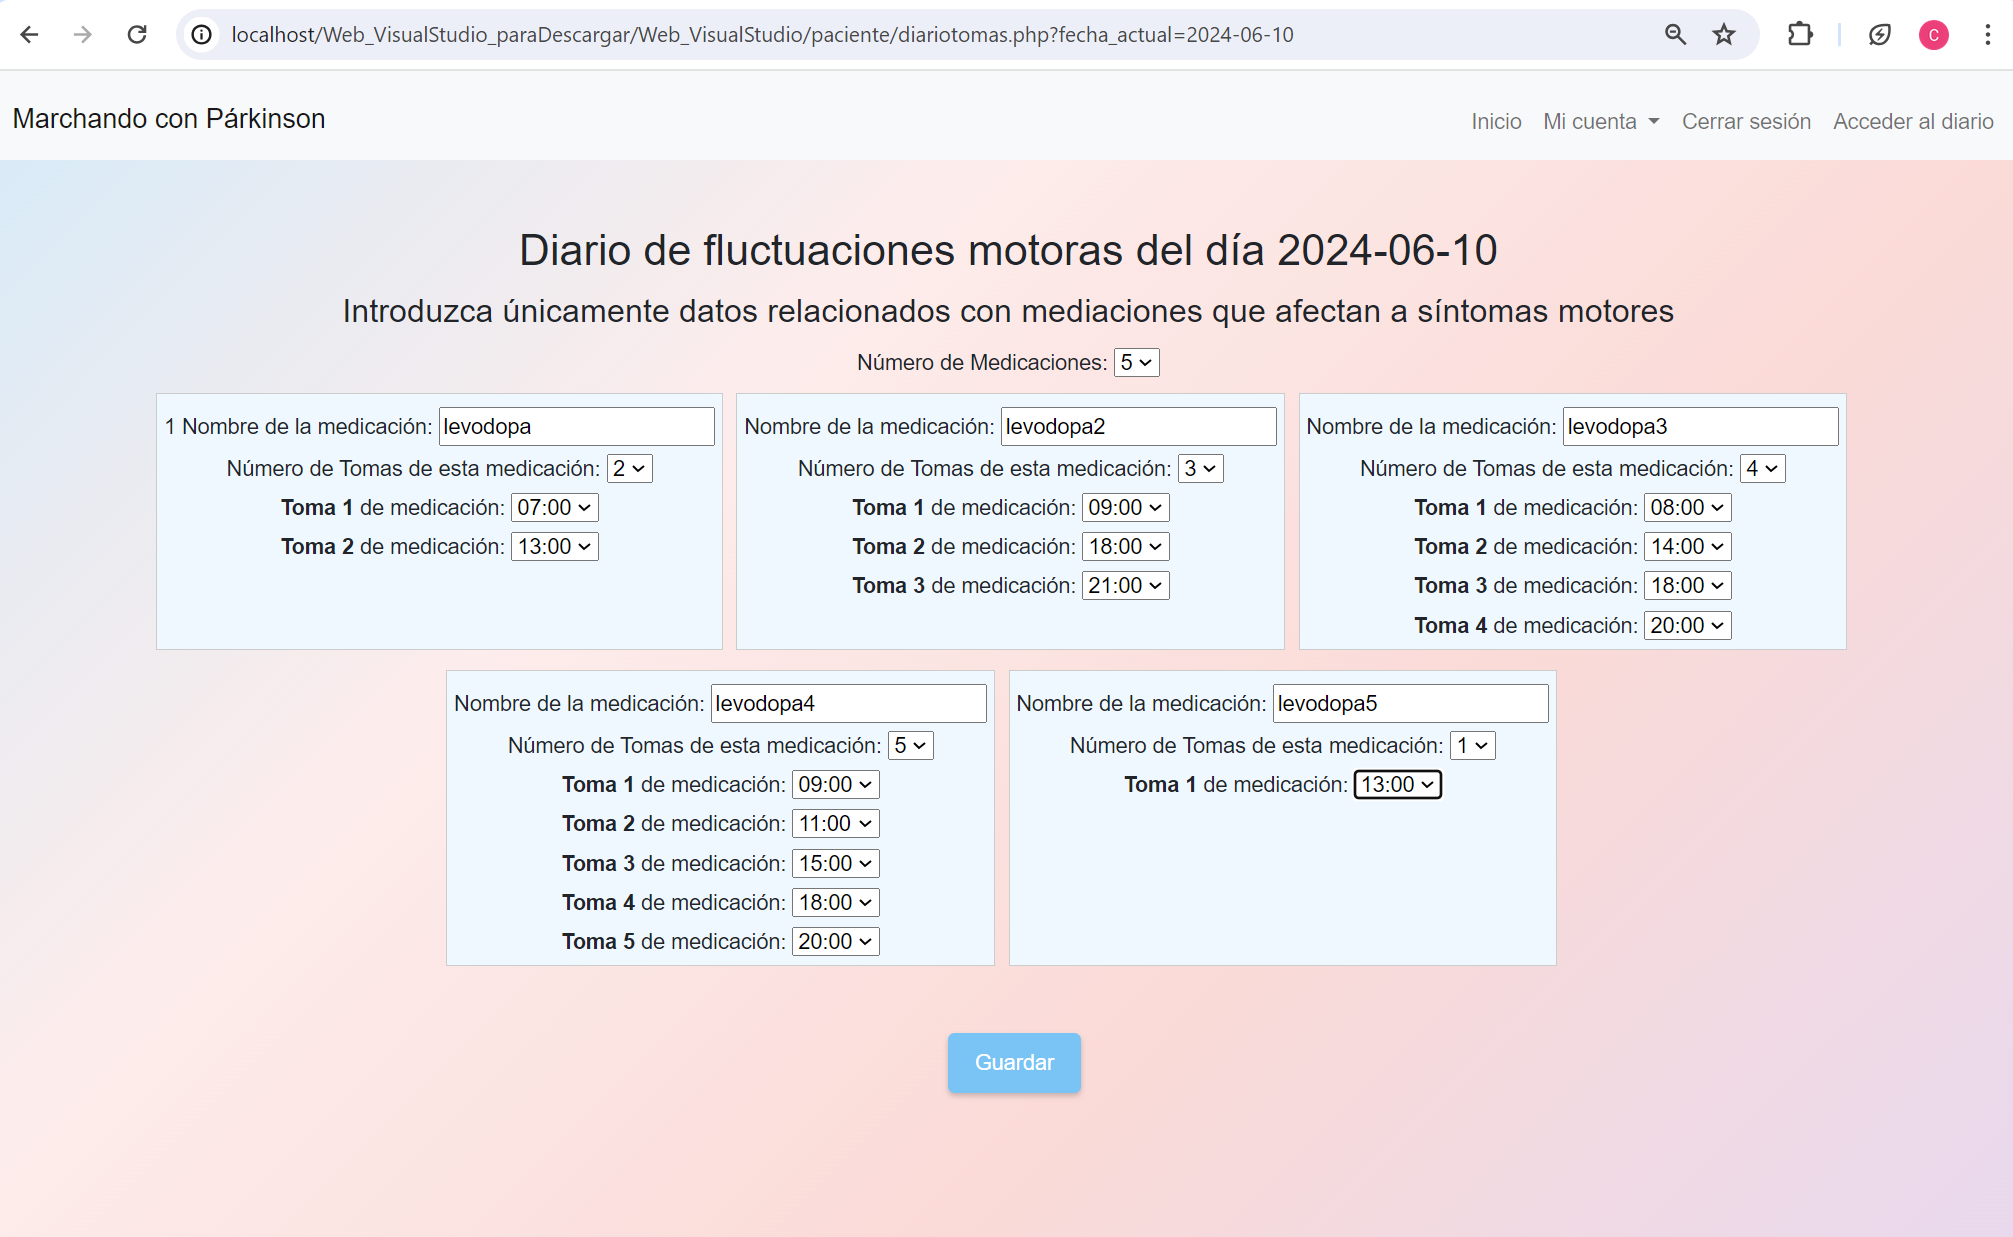
\includegraphics[width=1\textwidth]{img/diariotomas.png}
    \caption{Formulario para rellenar el diario de tomas de medicaciones. Fuente propia.}
    \label{fig:diariotomas}
\end{figure}
Adicionalmente, las funciones del usuario paciente incluyen la visualización de sus gráficas, de forma idéntica a la mostrada para el usuario profesional.
\subsection{Acceso a vídeos de funcionamiento de la aplicación web}
Dentro del repositorio GitHub utilizado, se puede acceder a los vídeos de demostraciones situados dentro de la carpeta 'Vídeos', donde se pueden observar con más detalle el funcionamiento y la demostración de las nuevas funciones de la aplicación.
     